%-------------------------------------------------------------------------------
%                            BAB III
%               		METODOLOGI PENELITIAN
%-------------------------------------------------------------------------------
\fancyhf{} 
\fancyfoot[C]{\thepage}
\chapter{METODOLOGI PENELITIAN}

\section{\uppercase{WAKTU DAN LOKASI PENELITIAN}}
Penelitian ini dilaksanakan di kota Banda Aceh. Waktu yang dibutuhkan untuk penelitian ini adalah 8 bulan, yang dimulai dari bulan November 2021 hingga Juni 2022.

% \section{\uppercase{JADWAL PELAKSANAAN PENELITIAN}}
% Jadwal pelaksanaan penelitian secara detail dapat dilihat pada Tabel \ref{tab:jadwal}

% \begin{table}[H]
% 	\begin{center}
% 	\caption{Jadwal Pelaksanaan Penelitian}
% 	\label{tab:jadwal}
% 	% \footnotesize
% 	\begin{tabular}{|c|l|c|c|c|c|c|c|c|c|}
% 	\hline
% 	\multirow{2}{*}{No.}&\multirow{2}{*}{Jenis Kegiatan}&\multicolumn{8}{c|}{Bulan}\\
% 	\cline{3-10}
% 	&&Nov&Des&Jan&Feb&Mar&Apr&Mei&Jun\\
% 	\hline
% 	1&Studi Literatur&\cellcolor{gray}&\cellcolor{gray}&&&&&&\\
% 	\hline
% 	2&Penulisan Proposal&&&\cellcolor{gray}&\cellcolor{gray}&&&&\\
% 	\hline
% 	3&Pengembangan Aplikasi&&&\cellcolor{gray}&\cellcolor{gray}&\cellcolor{gray}&&&\\
% 	\hline
% 	4&Evaluasi Sistem&&&&&&\cellcolor{gray}&\cellcolor{gray}&\\
% 	\hline
% 	5&Penulisan Laporan Akhir&&&&&&&&\cellcolor{gray}\\
% 	\hline
% 	\end{tabular}
% 	% \normalsize
% 	\end{center}
% \end{table}

\section{\uppercase{ALAT DAN BAHAN}}
Alat dan Bahan yang akan digunakan pada penelitian ini terdiri dari beberapa perangkat keras (\textit{hardware}) dan perangkat lunak (\textit{software}) yang dijabarkan sebagai berikut:

\begin{enumerate}
\item Perangkat Keras
	\begin{itemize}
	\item Laptop Dell Inspiron 15 7000 dengan spesifikasi RAM 12GB, Intel(R) Core(TM) i5-7300HQ CPU @2.5GHz, HDD 1TB dan SSD 250 GB.
	\end{itemize}

\item Perangkat Lunak
	\begin{itemize}
	\item Sistem Operasi Windows 10
	\item Figma
	\item Visual Studio Code v1.60.1
	\item XAMPP v3.2.4
	\item Brave Browser v1.29.81
	\item Potsman v8.10
	\end{itemize}
\end{enumerate}

\section{\uppercase{METODE PENELITIAN}}
Metode penelitian yang dilakukan akan terdiri dari beberapa tahapan. Skema dari alur tahapan tersebut dapat dilihat pada Gambar \ref{alur_penelitian}.

\begin{figure}[H]
\centering
{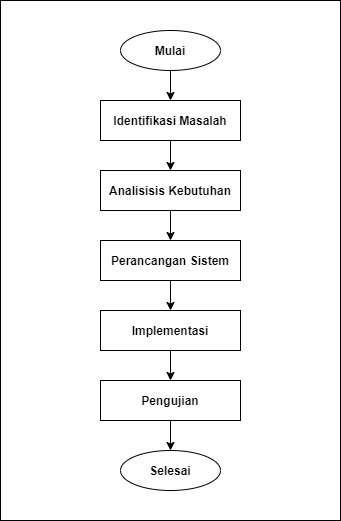
\includegraphics [width = 8cm, height= 11cm]{gambar/flowchart_proposal}}
\caption{Diagram Alir Penelitian}
\label{alur_penelitian}
\end{figure}

\par Adapun untuk metode pengembangan aplikasinya menggunakan metode pengembangan Scrum. Metode Scrum diimplementasikan pada tahapan analisis kebutuhan, perancangan sistem, implementasi, serta pengujian.

\fancyhf{} 
\fancyfoot[R]{\thepage}

\subsection{Identifikasi Masalah}
Tahapan ini merupakan tahapan yang dilakukan untuk mengidentifikasi masalah yang dihadapi pada sistem pemasaran saat ini, sehingga dari permasalahan yang didapatkan menjadi landasan untuk penelitian ini. Masalah-masalah yang berhasil diidentifikasi adalah sebagai berikut:

\begin{itemize}
	\item Sistem pemasaran saat ini masih dilakukan secara datang langsung ke tempat penjualan atau memesan lewat aplikasi media sosial.
	\item Pelanggan tidak dapat mengetahui ketersediaan stok produk sebelum bertanya kepada penjual atau mengunjungi langsung tempat penjualannya.
	\item Susahnya menjaga kestabilan harga produk antar penjual tanaman hidroponik.
\end{itemize}

\subsection{Analisis Kebutuhan}
Tahapan analisis kebutuhan dilakukan untuk mengetahui kebutuhan pengguna dan kebutuhan sistem serta fungsi apa saja yang akan dibangun nantinya didalam aplikasi. Kebutuhan tersebut dibagi menjadi dua yaitu kebutuhan fungsional yang mendefinisikan fungsionalitas dari sebuah sistem dan kebutuhan non-fungsional yang menjadi batasan kebutuhan yang tidak dapat dikerjakan oleh sistem itu sendiri. Setiap kebutuhan-kebutuhan tersebut akan dijabarkan sebagai berikut:

\begin{enumerate}[a.]
	\item Kebutuhan Fungsional
		\begin{itemize}
		\item Aplikasi berbasis web mampu mendaftarkan akun admin dan penjual.
		\item Aplikasi berbasis web mampu menampilkan jumlah dan informasi pengguna, produk, pesanan, ulasan dan laporan dari pembeli.
		\item Aplikasi berbasis web mampu mengelola promo dan produk seperti menambah, mengubah atau menghapus promo dan produk.
		\item Aplikasi berbasis web mampu memblokir penjual yang melakukan pelanggaran.
		\item Aplikasi berbasis web mampu meninjau pesanan yang masuk dari pembeli.
		\end{itemize}
	
	\item Kebutuhan Non-Fungsional
		\begin{itemize}
		\item Aplikasi berbasis web dapat diakses oleh superadmin, admin dan penjual dengan syarat adanya koneksi internet.
		\item Aplikasi berbasis web untuk saat ini hanya terbatas untuk wilayah kota Banda Aceh.
		\item Aplikasi berbasis web tidak dapat menerima pembayaran, karena pembayaran dilakukan secara tunai atau \textit{cash on delivery} (COD).
		\end{itemize}
	\end{enumerate}

% \par Melalui kebutuhan-kebutuhan di atas maka dibangunlah \textit{use case diagram} yang dapat dilihat pada gambar \ref{use_case_diagram}.

% \begin{figure}[H]
% 	\centering
% 	{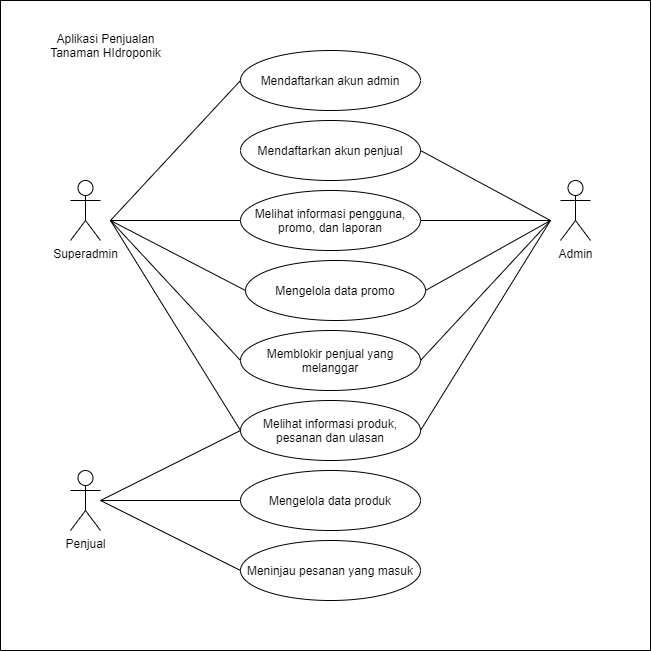
\includegraphics [width = 14cm, height= 14cm]{gambar/use_case_diagram}}
% 	\caption{Use Case Diagram}
% 	\label{use_case_diagram}
% \end{figure}

\subsection{Perancangan Sistem}
Tahap perancangan sistem dibuat berdasarkan hasil yang telah didapatkan dari analisis kebutuhan. Kemudian dirancang sistem agar dapat berjalan dengan baik, dimulai dari perancangan \textit{database} menggunakan \textit{Entity Relationship Diagram} (ERD), perancangan \textit{Business Diagram}, perancangan \textit{Activity Diagram} sampai rancangan alur kerja sistem. Alur kerja sistem dapat dilihat pada Gambar \ref{alur_kerja_sistem}.

% \textit{Business Diagram} dapat dilihat pada Gambar \ref{bisnis_diagram}.

% \begin{figure}[H]
% \centering
% {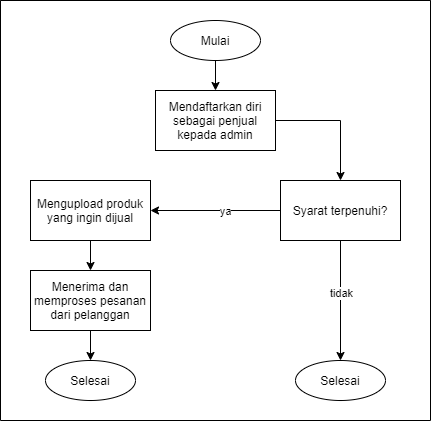
\includegraphics [width = 14cm, height= 10cm]{gambar/bisnis_diagram}}
% \caption{Business Diagram}
% \label{bisnis_diagram}
% \end{figure}

% Adapun alur kerja sistem dapat dilihat pada Gambar \ref{alur_kerja_sistem}.

\begin{figure}[H]
\centering
{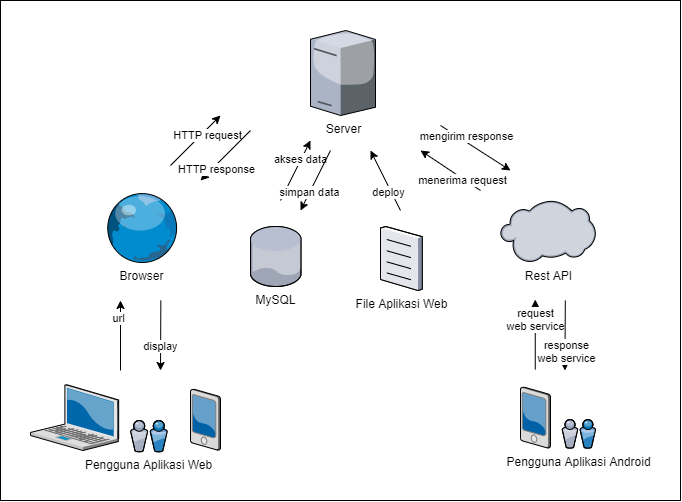
\includegraphics [width = 14cm, height= 10cm]{gambar/alur_kerja_sistem}}
\caption{Alur Kerja Sistem}
\label{alur_kerja_sistem}
\end{figure}

\subsection{Implementasi}
Setelah rancangan sistem selesai dilakukan, selanjutnya akan diimplementasikan hasil rancangan tersebut ke dalam bentuk kode pemrograman. Pada tahap ini aplikasi berbasis web akan dibangun menggunakan \textit{framework} Laravel dan MySQL sebagai \textit{database}. Selain Laravel juga digunakan \textit{library} tambahan di dalamnya yaitu Livewire. Livewire merupakan \textit{full-stack framework} untuk Laravel yang berguna untuk membuat tampilan antarmuka menjadi dinamis. Alasan penggunaan Livewire didalam penelitian ini supaya tidak perlu membuat terpisah antara \textit{front end} dan \textit{back end} sehingga akan mempercepat proses pengembangan aplikasi. Kemudian dari aplikasi web ini nantinya akan dibuatkan REST API untuk aplikasi Android agar dapat mengakses dan mengirimkan data ke dalam server.

\subsection{Pengujian}
Pengujian sistem sangat diperlukan untuk memastikan sistem yang sudah dibangun dapat berjalan sesuai dengan apa yang diharapkan. Pada penelitian ini akan dilakukan 2 pengujian yaitu pengujian fungsionalitas dan pengujian \textit{usability}.

\begin{enumerate}
	\pagebreak
	\item Pengujian Fungsionalitas
	\par Pengujian Fungsionalitas dilakukan dengan menggunakan metode \textit{Black Box}. Metode ini berfokus pada fungsionalitas dari aplikasi yang telah dibuat dengan cara menguji aplikasi tersebut apakah sudah berjalan sesuai yang diharapkan atau belum, seperti menguji fungsi-fungsi pada aplikasinya, \textit{input output} yang dihasilkan, serta dalam mengakses data.
	\item Pengujian \textit{Usability}
	\par Pengujian \textit{Usability} dilakukan dengan menggunakan metode \textit{Usability Metric for User Experience} (UMUX). Pengujian ini dilakukan untuk menguji aplikasi yang sudah dibuat apakah sudah sesuai dengan kebutuhan pengguna serta mudah untuk digunakan dan dipahami oleh pengguna aplikasi. Pengujian akan dilakukan dengan membagikan kuesioner kepada beberapa sampel pengguna yang akan menggunakan aplikasi. Nantinya dari hasil kuesioner tersebut akan didapatkan hasil apakah aplikasi dikatakan layak digunakan atau tidak. 
\end{enumerate}

%-----------------------------------------------------------------------------%

% Baris ini digunakan untuk membantu dalam melakukan sitasi
% Karena diapit dengan comment, maka baris ini akan diabaikan
% oleh compiler LaTeX.
\begin{comment}
\bibliography{daftar-pustaka}
\end{comment}